\documentclass[../thesis.tex]{subfiles}

\begin{document}

\chapter{Benchmark}
\label{chap:bm}

\section{Aim}
The aim of benchmarking is understanding the performance characteristics of the proposed system under various loads and system configurations.

\section{Setup}

The hardware used for benchmarking is detailed in \autoref{sec:benchmarkingServer} and the critical technical specifications that affect the performance of the system are:
\begin{itemize}
\item 8 Core 16 Threads
\item 4.3 GHz Clock Speed
\item 32 GB Memory
\item Hardware Virtualisation Enabled
\end{itemize}

To observe the performance characteristics of the proposed system with horizontal scalling, additional hardwares used for horizontal scalling benchmarking are listed below:
\begin{itemize}
\item MacBook Pro 16 2019
\begin{itemize}
\item 8 Core 16 Threads
\end{itemize}
\item HP Envy dv6 2013
\begin{itemize}
\item 4 Core 8 Threads
\end{itemize}
\end{itemize}


The software used for benchmarking is detailed in \autoref{sec:software} and the critical technical specifications are:
\begin{itemize}
\item Ubuntu 20.04
\item Docker Engine Enabled
\end{itemize}

Additionally, the proposed system has two configurations that can be tweaked to show how the performance can be impacted:

\begin{itemize}
\item Number of backend instances
\item Number of async workers
\end{itemize}

The components of the proposed system are deployed to the benchmarking server using Docker Containers\footnote{A container virtualisation method, which allows the components to be run in an isolated environment that is always identical regardless of the environments of the server.} to manage the runtime dependencies. Note that this method of deployment has minimal impact on the performance of the system.

\subsection{Limited Computational Resources}
The configurations listed in the table \ref{tab:lowsysconfbench} are used to observe the behaviours of the proposed system with limited computation resources that is comparable to a modern laptop.

\begin{table}[h!]
\begin{center}
\caption{A set of system configurations used for performance benchmarking with limited computational resources.}
\label{tab:lowsysconfbench}
\begin{tabular}{l|l|l}
\toprule
\textbf{No. Backend Instances} & \textbf{No. Async Workers} & \textbf{No. Devices}\\
\midrule
4 & 4 & 50\\
4 & 4 & 100\\
4 & 4 & 200\\
\bottomrule
\end{tabular}
\end{center}
\end{table}

\subsection{Reasonable Computational Resources}

The configurations listed in the table \ref{tab:highsysconfbench} are used to observe the behaviours of the proposed system with reasonable computation resources that are comparable to a high-performance consumer-grade desktop computer system.

\begin{table}[h!]
\begin{center}
\caption{A set of system configurations used for performance benchmarking with reasonable computational resources.}
\label{tab:highsysconfbench}
\begin{tabular}{l|l|l}
\toprule
\textbf{No. Backend Instances} & \textbf{No. Async Workers} & \textbf{No. Devices}\\
\midrule
4 & 12 & 100\\
4 & 12 & 200\\
\bottomrule
\end{tabular}
\end{center}
\end{table}

\subsection{Horizontal Scalling}

The proposed system is designed to scale, that is, having the capability of running multiple instances on multiple servers to distribute the load. The table \ref{tab:scalebench} shows the configurations used for benchmarking where there are three physically separated servers contributing to executing the tasks at the same time. The computation resources provided by the servers are shown in the table \ref{tab:computecontrib}

\begin{table}[h!]
\begin{center}
\caption{Contribution to computational resources.}
\label{tab:computecontrib}
\begin{tabular}{l|l|l|l}
\toprule
\textbf{Server} & \textbf{Threads} & \textbf{No. Backend} & \textbf{No. Workers}\\
\midrule
Benchmarking Server & 16 & 8 & 8\\
MacBook Pro 16 2019 & 16 & 0 & 8\\
HP Envy dv6 2013 & 8 & 0 & 8\\
\bottomrule
\end{tabular}
\end{center}
\end{table}

\begin{table}[h!]
\begin{center}
\caption{A set of system configurations used for scalability benchmarking.}
\label{tab:scalebench}
\begin{tabular}{l|l|l}
\toprule
\textbf{No. Backend Instances} & \textbf{No. Async Workers} & \textbf{No. Devices}\\
\midrule
4 & 8 + 8 + 8 & 200\\
4 & 8 + 8 + 8 & 500\\
\bottomrule
\end{tabular}
\end{center}
\end{table}

\section{Procedures}

\subsection{Generating Loads}

The simulator is used to generate realistic loads by spawning computer processes that are accessing the backend in the same manner as a real remote sensing device. For each simulated remote sensing device, it sends the sensing data to the backend every second for a total of 500 iterations\footnote{One iteration means sending data to the backend one time.} to create a sustained load.

To verify the simulator is performing normally, that is, the simulator is generating the expected sustained load. A timer is used to verify if the simulator terminates within the expected time interval. In the benchmarking, the timer is set to 8.3 minutes\footnote{500 Requests / 60 Requests Per Minute = 8.3 Minutes}. This is because when the total number of requests are the same, then terminating later than expected means the number of requests per minute is lower the expected value, which means a lighter load is generated. This can be an indication of the number of simulated devices are beyond the capability of the benchmarking server. In which case, the result is discarded.


\subsection{Measuring Performance}

To quantify the performance, the response time of each request is measured and recorded. Once a simulated device has finished sending data, the response time for each iteration is saved to a CSV (Comma Separated Values) file. Once all simulated devices have finished sending data, the average response time for each iteration across all simulated devices is calculated and saved to another CSV file. This is used to determine how well the backend handles various loads.

The monitoring delay is the time it takes from recording the data in the sensing device to showing the data on the client. In the benchmarking, the delay can be measured by the time duration between the termination of the last simulated device and receiving the last data update. If the last simulated device terminated at around the same time as the last data update, then the system is keeping up with the load. If the last data update is received significantly later than the termination of the last simulated device, then it must indicate the system cannot keep up with the number of data updates.


\section{Analysis}

\subsection{Limited Computational Resources}

The average response time under different loads with limited computational resources is shown in the table \ref{tab:avg4-4}. From the table, it is clear the given loads did not saturate the backend since the response time for each load is considered very short. It is worth noting the response time slightly increases as the number of devices increases, which is expected.

\begin{table}[h!]
\begin{center}
\caption{The average response time for the 4 backends and 4 async workers configuration.}
\label{tab:avg4-4}
\begin{tabular}{l|l}
\toprule
\textbf{No. Devs} & \textbf{Average Response Time}\\
\midrule
50 & 4.03 milliseconds\\
100 & 4.87 milliseconds\\
200 & 5.26 milliseconds\\
\bottomrule
\end{tabular}
\end{center}
\end{table}

The monitoring delay with limited computational resources is shown in the table \ref{tab:delay4-4}. There is no delay for the load of 50 devices. However, the load of 100 devices introduced a 4 minutes delay and the load of 200 devices introduced a 16 minutes delay. That means, it takes minutes for new data to show up on the client after it is recorded at the sensing device. Because the backend is nowhere near its saturation point as evidenced by the short response time. The only bottleneck is the four async workers are struggling to process the amount of data insertion requests in the job queue. This is because the data insertion requests are handled by the async workers, not the backend itself, as inserting data into the database is considered time-insensitive in this scenario. Additionally, the data updates are only generated until the async worker successfully insert the data into the database, which explains the significant delay in receiving updates at the clients.

\begin{table}[h!]
\begin{center}
\caption{The monitoring delay for the 4 backends and 4 async workers configuration.}
\label{tab:delay4-4}
\begin{tabular}{l|l}
\toprule
\textbf{No. Devs} & \textbf{Delay}\\
\midrule
50 & No delay \\
100 & 4 Mins\\
200 & 16 Mins\\
\bottomrule
\end{tabular}
\end{center}
\end{table}

Figure \ref{fig:4-4} shows the response time for each iteration under different load scenarios. The figure suggests there are no positive or negative associations between the response time and the number of iterations. That means the response time is expected to stay at the same level as the number of iterations approaches infinite.

\begin{figure}[!ht]
\centering
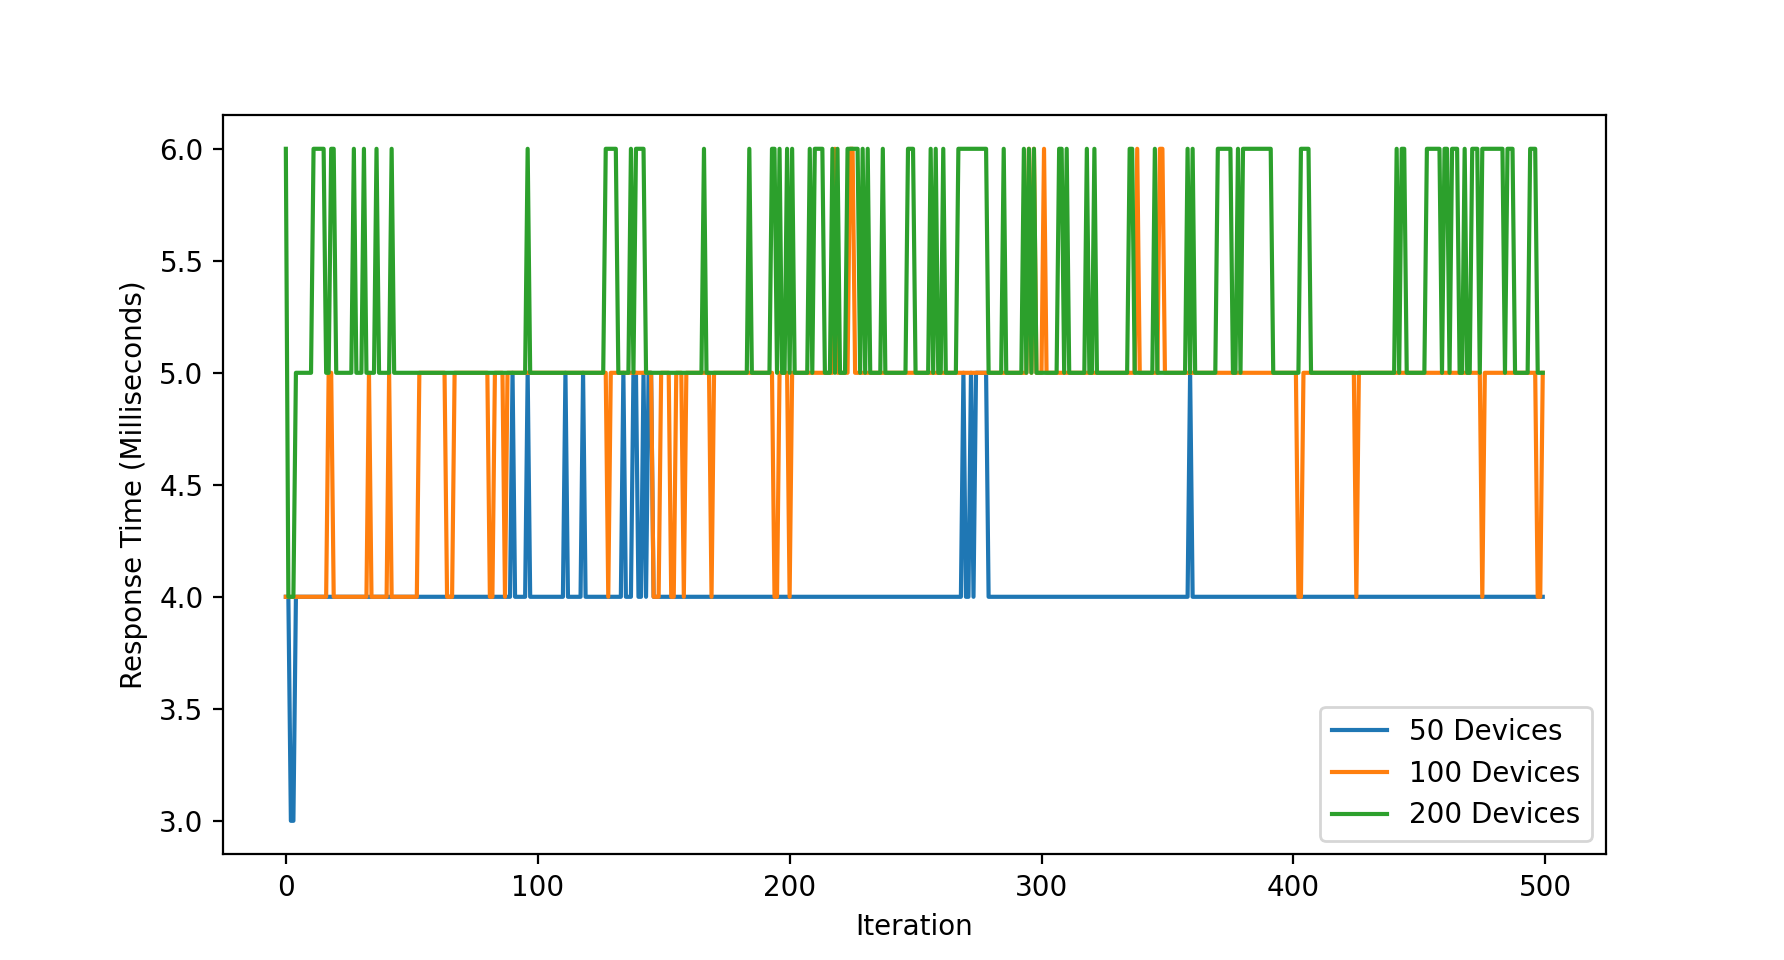
\includegraphics[width=\linewidth]{4-4.png}
\caption{The response time for each iteration using the 4 backends and 4 async workers configuration.}
\label{fig:4-4}
\end{figure}

With the evidence presented above, the 4 backends and 4 async workers configuration, which is comparable to the performance of a laptop, is expected to serve around 50 devices for a long period without introducing delays or significant performance degradation. Since 4 async workers are bottlenecking the system, then increasing number of async workers should improve the performance significantly, which is discussed in the \autoref{sec:reasonable} where 8 additional workers are added to the system.

\subsection{Reasonable Computational Resources}
\label{sec:reasonable}
The average response time under different loads with reasonable computational resources is shown in the table \ref{tab:avg4-12}. The response time of the backend with reasonable computational resources performs similarly to the backend with limited computational resources. They are considered short and shows no sign of saturating the throughput of the backend.

\begin{table}[h!]
\begin{center}
\caption{The average response time for the 4 backends and 12 async workers configuration.}
\label{tab:avg4-12}
\begin{tabular}{l|l}
\toprule
\textbf{No. Devs} & \textbf{Average Response Time}\\
\midrule
100 & 4.46 milliseconds\\
200 & 7.75 milliseconds\\
\bottomrule
\end{tabular}
\end{center}
\end{table}

The delay tells a very different story, which is shown in the table \ref{tab:delay4-12}. There is no longer any delay with 100 devices, which is improved by 4 minutes. The 16 minutes delay with 200 devices is reduced to 5 minutes. The significant improvements are coming from the additional 8 workers performing data insertion requests in parallel. The total of 12 async workers can process a lot more requests than the 4 async workers, thus keeping up with the load generated by the 100 devices. However, the 12 async workers are still not processing the data insertion requests fast enough causing a significant delay with 200 devices. More importantly, the available computational resources on the benchmarking server are fully occupied and no more useful resources can be allocated in executing the data insertion requests from the benchmarking server. Fortunately, the solution to this problem is using a technique called horizontal scaling, which is discussed in \autoref{sec:horizontal}.

\begin{table}[h!]
\begin{center}
\caption{The monitoring delay for the 4 backends and 12 async workers configuration.}
\label{tab:delay4-12}
\begin{tabular}{l|l|l}
\toprule
\textbf{No. Devs} & \textbf{Delay} & \textbf{Improvement}\\
\midrule
100 & No delays & 4 Mins	\\
200 & 5 Mins & 11 Mins\\
\bottomrule
\end{tabular}
\end{center}
\end{table}

Figure \ref{fig:4-12} shows the response time for each iteration under different load scenarios. Similar to before, there are no signs that indicate the response time will increase nor decrease as the number of iterations increases. Which means the response time is likely to stay at the same level as the number of iterations approaches infinite. An interesting observation in the figure is the periodic fluctuations in the response time which happens every 60 to 80 iterations. More discussion about the fluctuations and probable causes can be found in \autoref{sec:horizontal}.

\begin{figure}[!ht]
\centering
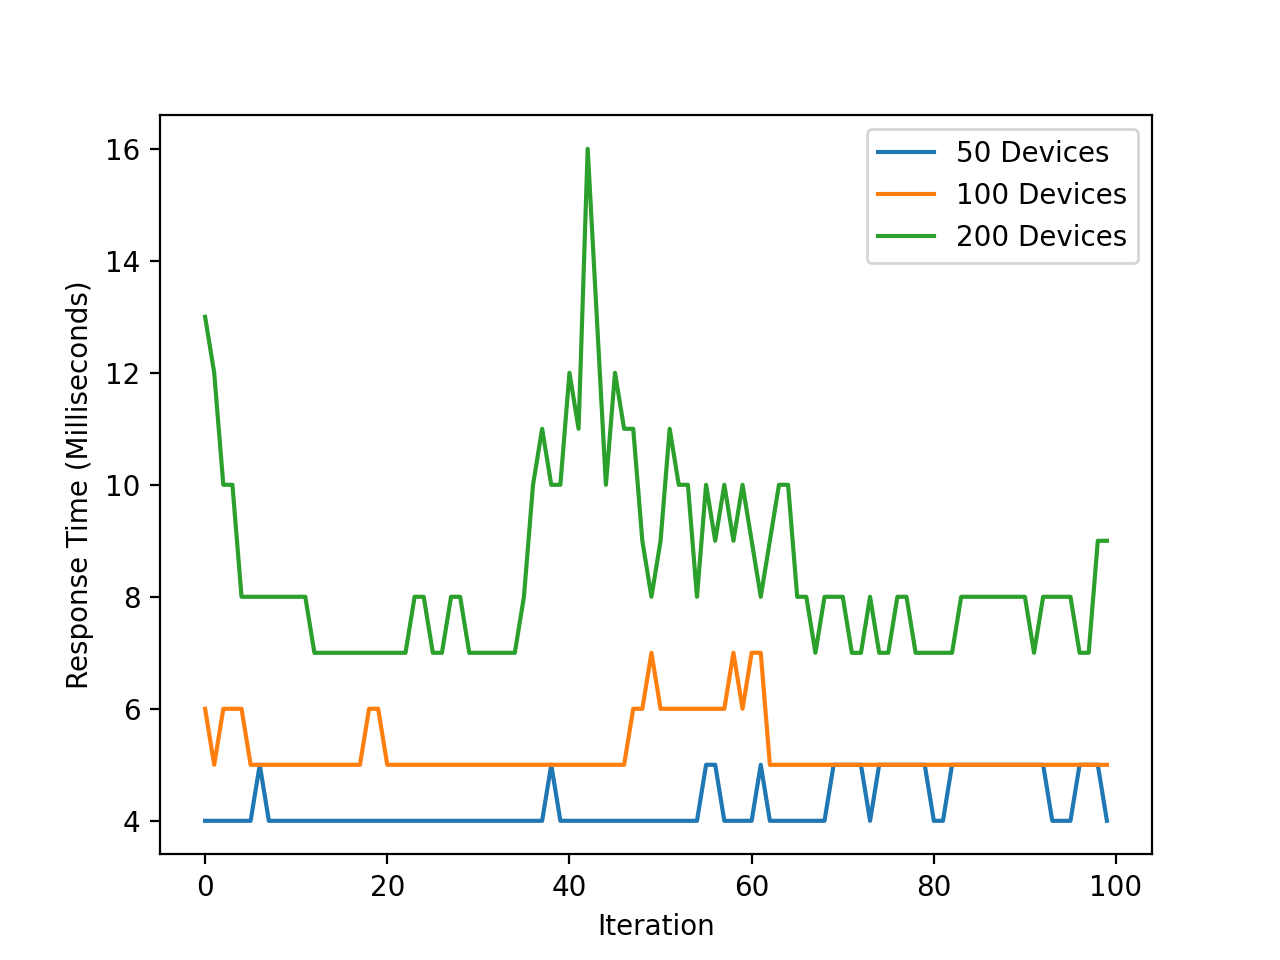
\includegraphics[width=\linewidth]{4-12.png}
\caption{The response time for each iteration using the 4 backend and 12 async worker configuration.}
\label{fig:4-12}
\end{figure}

In summary, the additional 8 workers improved the performance of the server significantly by removing bottlenecks. The system with reasonable computational resources that is comparable to a high-end consumer-grade desktop computer is capable of serving 100 devices gracefully. However, the bottleneck still exists and more async workers are needed to handle the demanding situations.

\subsection{Horizontal Scalling}
\label{sec:horizontal}

The horizontal scaling enables separate servers contributing to the processing of requests. The average response time under different loads with light horizontal scaling is shown in the table \ref{tab:avg8-24}. The load from 200 devices is still being handled gracefully with an increase in 4 extra backend instances, as expected. However, the load from 500 devices overwhelms some parts of the system as evidenced by the unusually long response time. As we will discover in the later discussion, the potential bottlenecking is not likely to be the backend but the job queue.

\begin{table}[h!]
\begin{center}
\caption{The average response time for the 8 backends and 24 async workers configuration.}
\label{tab:avg8-24}
\begin{tabular}{l|l}
\toprule
\textbf{No. Devs} & \textbf{Average Response Time}\\
\midrule
200 & 6.31 milliseconds\\
500 & 178.66 milliseconds\\
\bottomrule
\end{tabular}
\end{center}
\end{table}

The table \ref{tab:delay8-24} shows the delays with various load scenarios. The good news is a total of 16 async workers had been able to keep up with the load from 200 devices. The significances of the 16 async workers are they are not coming from the same server. Instead, they are running on three physically separated servers, and interact and distribute loads with each other through the internet. This implies the proposed system can be easily scaled up and down depending on the number of panels that are being monitored. Unfortunately, the 16 async workers are still not fast enough to keep up with the load from 500 devices with a significant 11 minutes delay.

\begin{table}[h!]
\begin{center}
\caption{The monitoring delay for the 8 backends and 24 async workers configuration.}
\label{tab:delay8-24}
\begin{tabular}{l|l|l}
\toprule
\textbf{No. Devs} & \textbf{Delay} & \textbf{Improvement}\\
\midrule
200 & No delays & 5 Mins	\\
500 & 11 Mins & N/A\\
\bottomrule
\end{tabular}
\end{center}
\end{table}



In figure \ref{fig:w-4-12-24}, the response time for each iteration under the load of 200 devices with different configurations are shown. Under the same amount of load and the same amount of backend instances, the 4-4 (4 Backend 4 Workers) configuration have much smaller fluctuations than the 4-12 (4 backends 12 workers) configuration. The only difference is the 4-4 configuration have 8 threads that are free to be utilised by the job queue and databases, whereas the 4-12 configuration have no dedicated threads for the job queue and databases. Since the number of backend instances remains the same but the fluctuation is reduced by having dedicated threads for job queue and databases, it suggests the performance of the job queue and databases is severely impacted by the limited computational resources in the 4-12 configuration.

\begin{figure}[!ht]
\centering
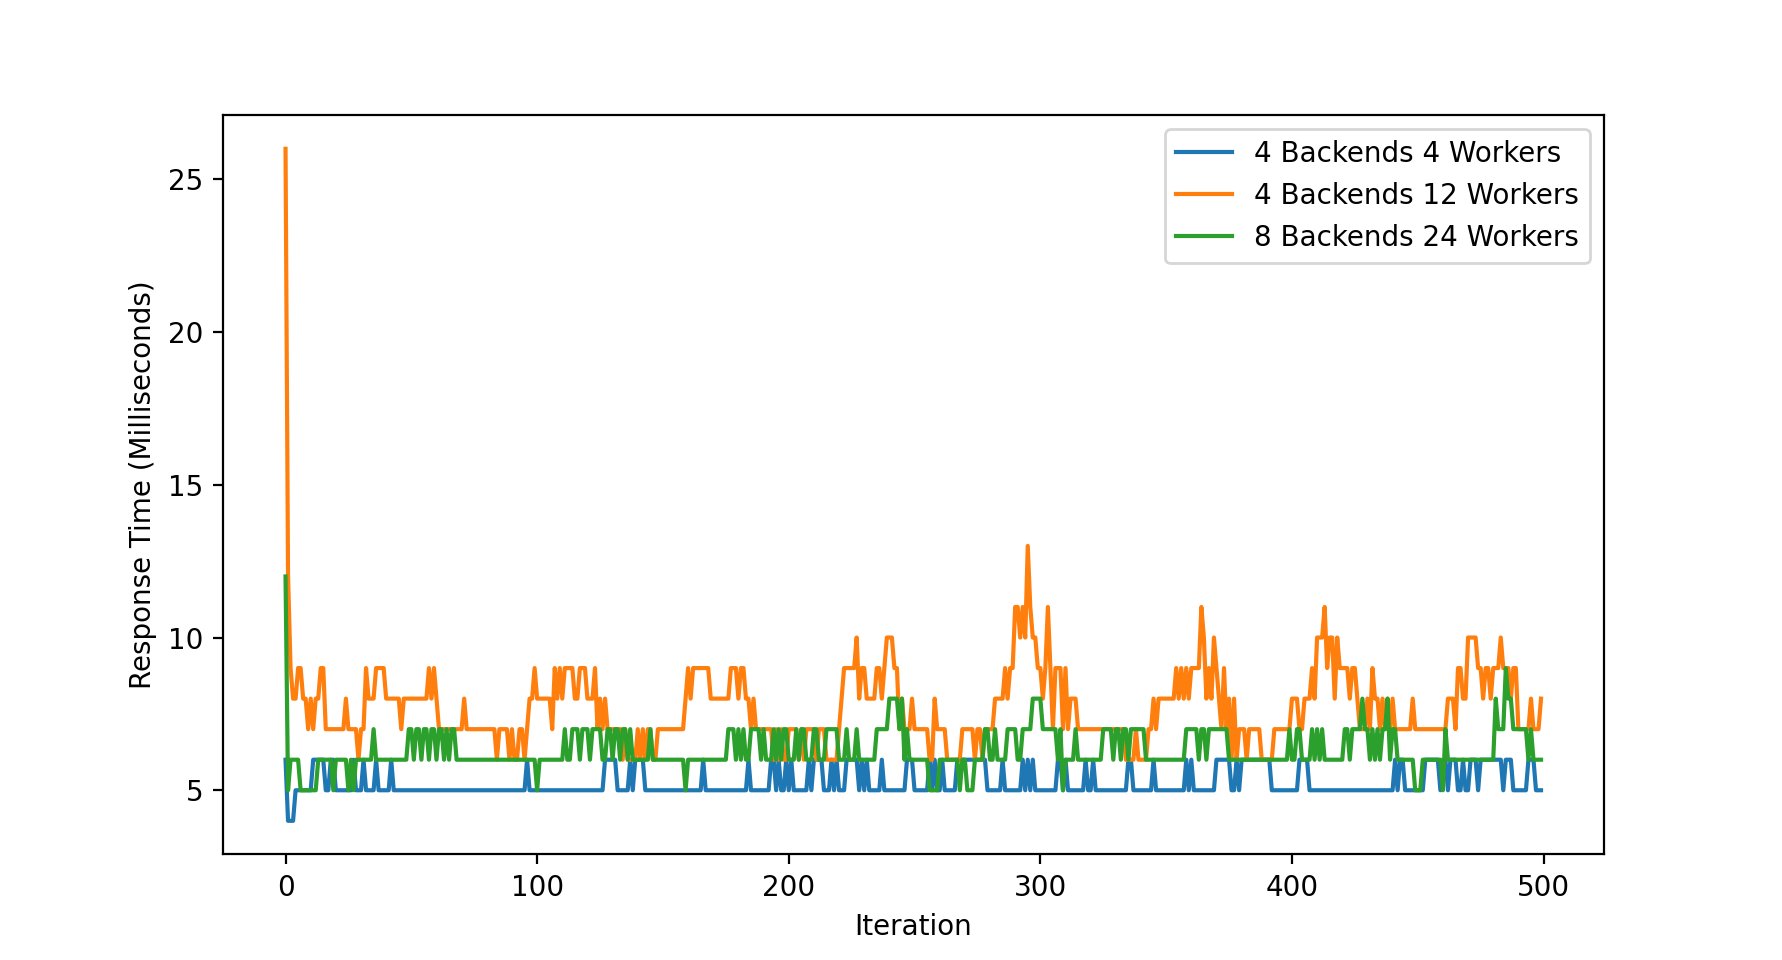
\includegraphics[width=\linewidth]{w-4-12-24.png}
\caption{The response time for each iteration with 200 devices in all configurations.}
\label{fig:w-4-12-24}
\end{figure}


The figure \ref{fig:8-24} shows the response time for each iteration under different load scenarios. The fluctuations of the response time under the load of 500 devices can be as long as 380 milliseconds. This is an indication of a bottleneck exists in the system. Because the fluctuations are caused by the job queue and databases not having enough computational resources to keep up with the demand. The bottleneck is likely to be resolved by giving the job queue and database more computational resources such as dedicated threads.

\begin{figure}[!ht]
\centering
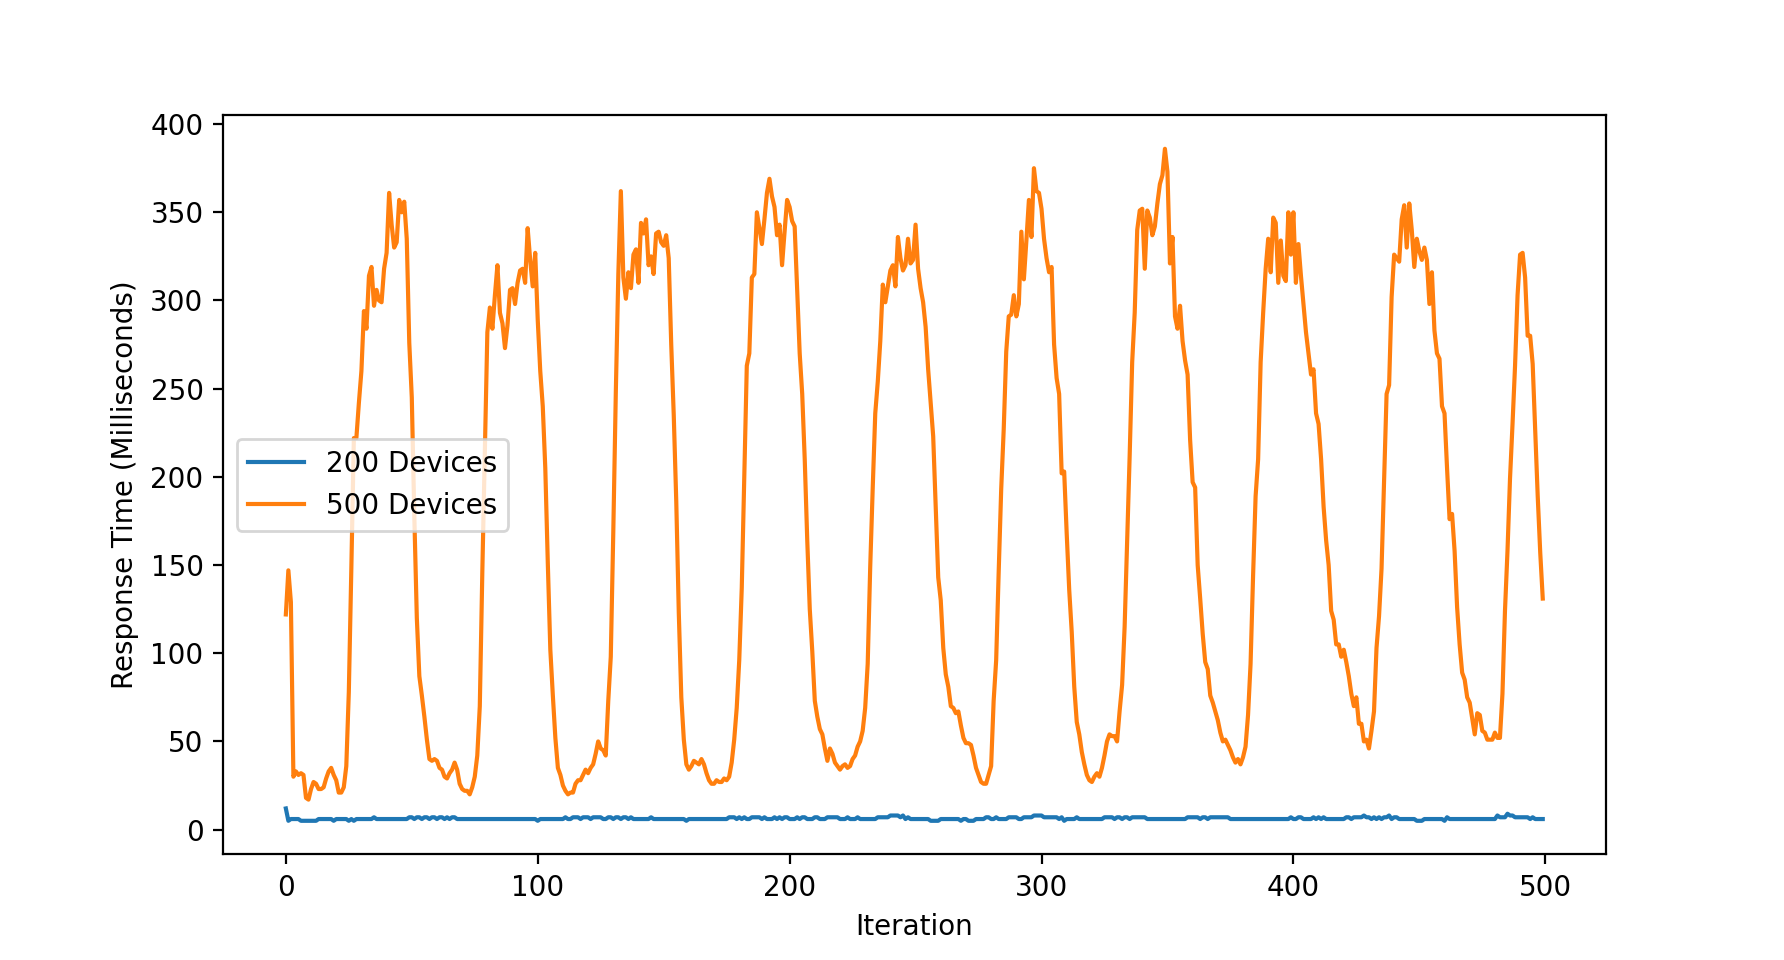
\includegraphics[width=\linewidth]{8-24.png}
\caption{The response time for each iteration using the 4 backend and 8 + 8 + 8 async worker configuration.}
\label{fig:8-24}
\end{figure}

The figure \ref{fig:jq-bottle} shows the results of different attempts at minimising the bottlenecks. The response time is measured by simulating 300 devices making 100 requests each. The 2 free threads with 1 job queue configuration are the baseline performance, and it is the same configuration that we used above. With this configuration, The peak response time reaches 160 milliseconds, which is very slow. The first attempt is increasing the number of job queues from one to two so that the load is distributed over two separate job queues. The effect of using more job queues is it greatly improves the peak response time and takes longer to reach the peak response time. However, the response time can still be around 100 milliseconds when the queues are nearing its full capacity. The second attempt is increasing the number of dedicated threads that can be utilised by the job queue from 2 to 4. As shown in the figure, the peak response time drops to acceptable 60 milliseconds. This further shows the proposed system is very scalable to accommodate the different amount of loads.

\begin{figure}[!ht]
\centering
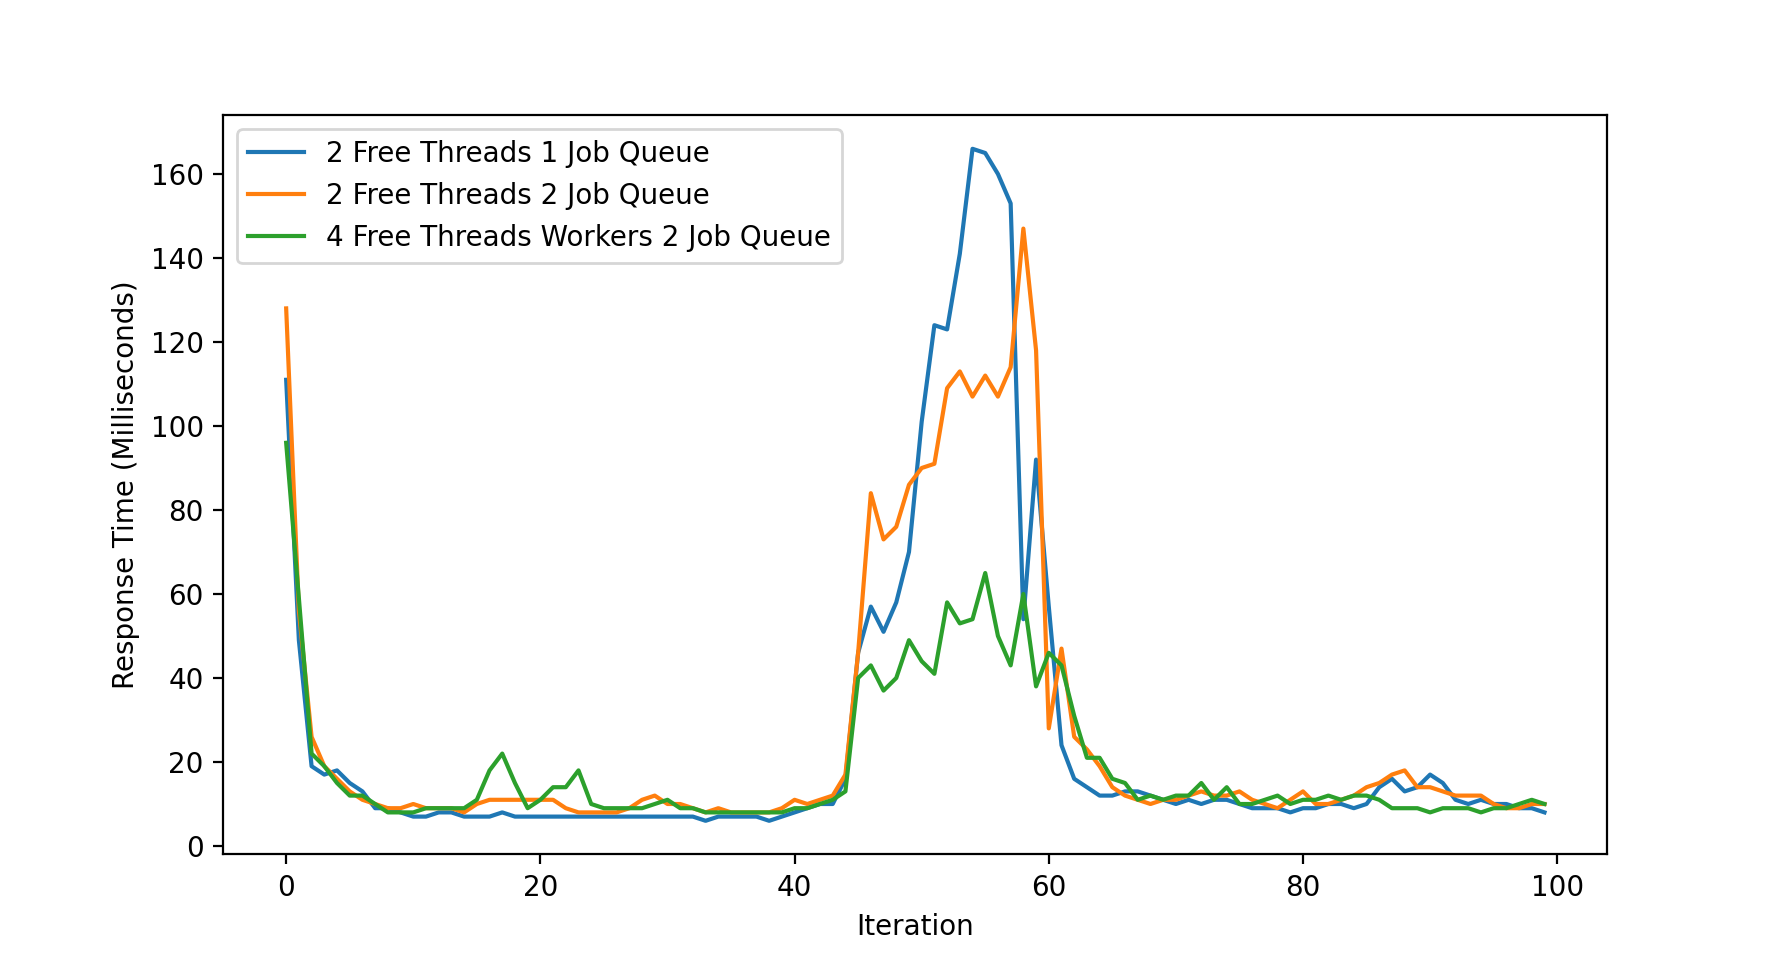
\includegraphics[width=\linewidth]{jq-bottle.png}
\caption{The response time for each iteration with different job queue scaling and avaliable resources.}
\label{fig:jq-bottle}
\end{figure}


The fluctuation is very likely to be caused by the job queue under the impact of limited computational resources. It is likely suffering from slow memory allocation when the job queue is nearing its full capacity and it needs to find more space to store the tasks. When the job queue has plenty of space remaining, the job can be added immediately, which has a lower response time. As the queue is about to full, and the slow memory allocation cannot keep up with the incoming jobs, the response time is significantly increased as it is waiting for free space to be available in the queue. Once the memory allocation is completed, there is plenty of space left, the response time drops again. This process is repeated again and again, causing fluctuations.

\subsection{Batch Processing}

In the previous section where horizontal scaling is tested and we see some big improvements. The problem with the previous approach is it aims to achieve the best performance by using a lot of computational resources. For example, handling the data insertion request individually. This approach means the number of jobs in the job queue positively proportional to the number of devices in the system, which implies the number of workers is positively proportional to the number of devices as well. This is fine if we have a lot of computational resources to scale up the system, but that is not always the case. In which case, compromises have to be made to accommodate situations where computational resources are limited.

As we have found out that one of the limiting factors is how many data insertion requests the system can handle, that means we can attempt to reduce the number of requests in the system to improve the performance. Batch processing is a simple idea where many data insertion requests are buffered somewhere in the system and then inserted altogether. The tradeoff of this approach is the data update is no longer instantaneous but delayed for at most one second due to buffering. The benefit of this approach is decoupling the number of data insertion requests in the job queue from the number of devices. That is, with batch processing, there are at most one data insertion request performing all data insertions every second.

One of the main reason the batch processing can insert the same amount of data much faster and less demanding is that each data insertion request has to establish a connection with the database. If there are many data insertion requests, that means there is a huge overhead at establishing a new connection every time. In batch processing, there is only one request inserting a large batch of data, which reduces the number of times it needs to establish a new connection for inserting the same amount of data.

The batch processing benchmark is performed with the configuration detailed in the table \ref{tab:batch}

\begin{table}[h!]
\begin{center}
\caption{The batch processing benchmarking configuration.}
\label{tab:batch}
\begin{tabular}{l|l|l|l|l}
\toprule
\textbf{Backends} & \textbf{Workers} & \textbf{Free Threads} & \textbf{NO. Devices}\\
\midrule
6 & 8 & 2 & 1000\\
\bottomrule
\end{tabular}
\end{center}
\end{table}

During the benchmark, each device performs 100 iterations of data insertion and the response time of each iteration is measured. The average response time of each iteration across devices is shown in figure \ref{fig:batch}. Despite the average response time of each iteration is relatively slow, the batch processing enables the system to handle 1000 devices with no prolonged monitoring delay at all. The improvement comparing to the previous approach is 800 extra devices.

\begin{figure}[!ht]
\centering
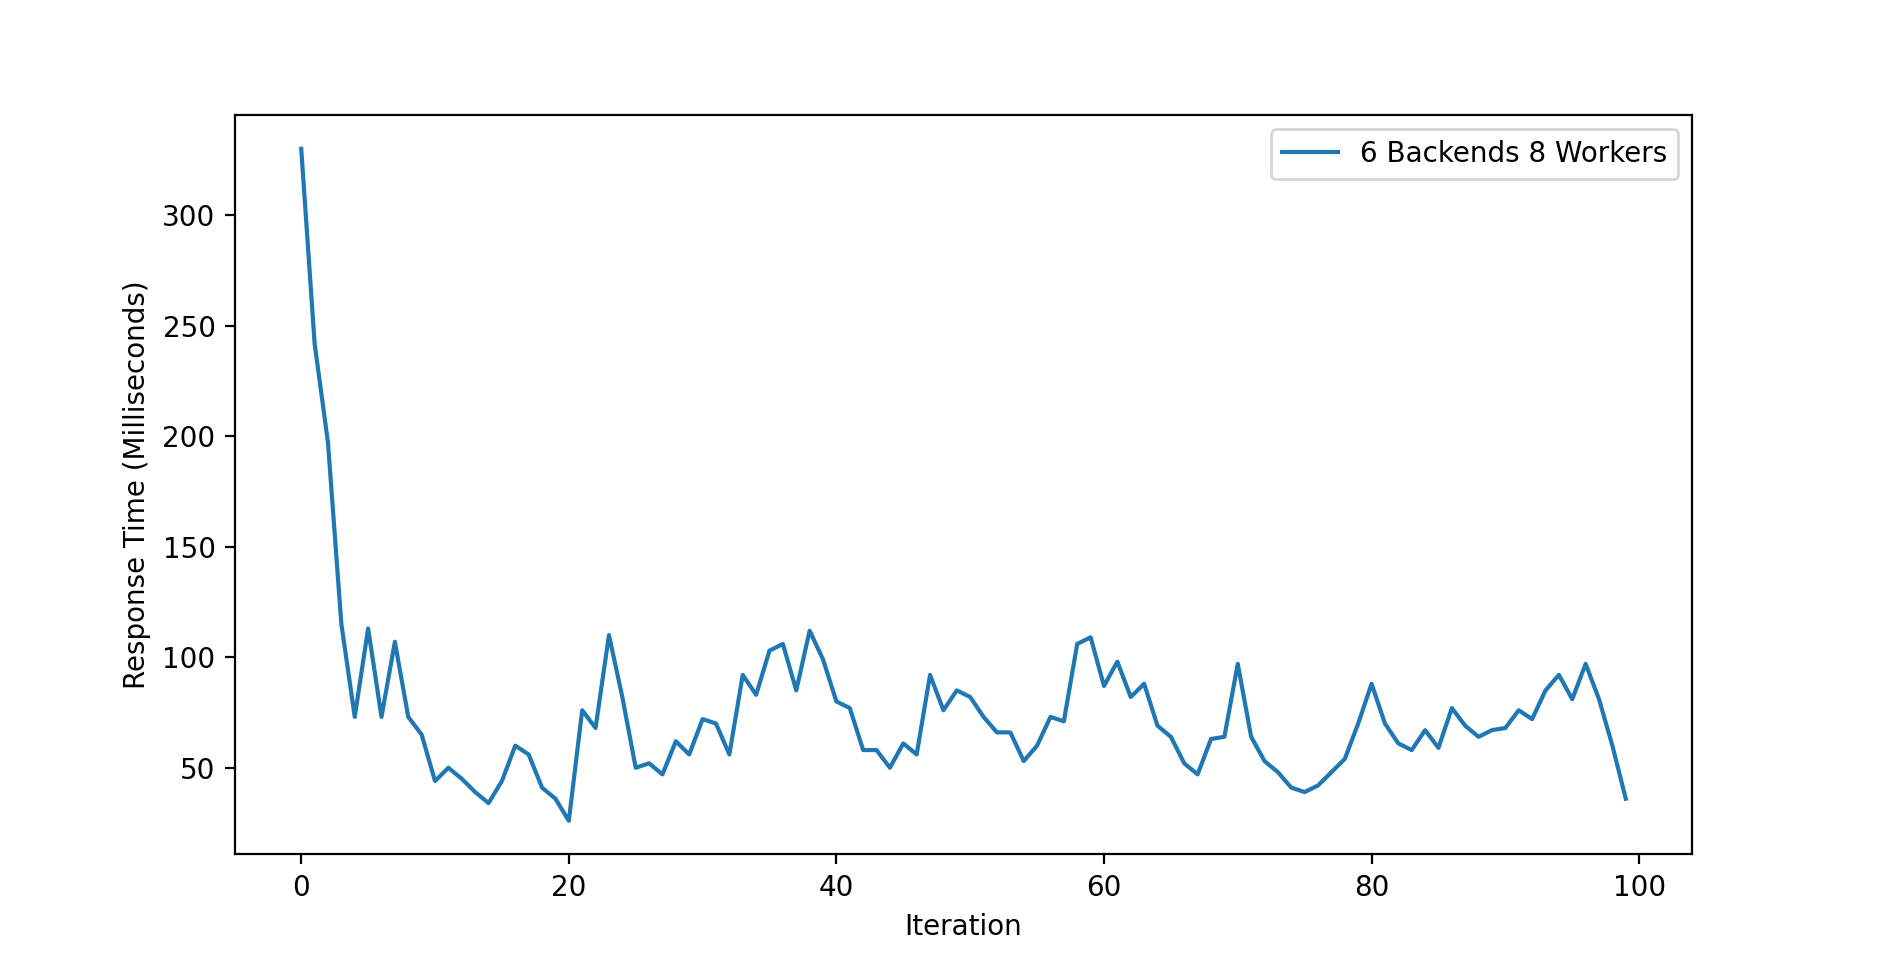
\includegraphics[width=\linewidth]{batch1000.png}
\caption{The response time for each iteration using batch processing.}
\label{fig:batch}
\end{figure}

\end{document}